%!TeX root=../index.tex

\section{Einleitung}\label{sec:introduction}

Der folgende Text dient der Dokumentation eines Programmierprojekts, welches im Rahmen der Vorlesung \texttt{TM40401.1 Mobile Computing} durchgeführt wurde.
Es galt mittels des Frameworks \emph{flutter}\footnote{\url{https://flutter.dev/}} eine Mobile-App zu entwickeln, welche Kindern (im Alter von ca. 6--8) das kleine Einmaleins beizubringen.

% Zusammenfassung

% Struktur

\section{Methode}

\subsection{Grundannahmen}

Abgeleitet von der Zielgruppe---Kinder im Alter von ca. 6--8 Jahren---habe ich zunächst einige Grundannahmen abgeleitet, was die Gestaltung der Lernfunktion angeht.
Kinder in diesem Alter haben nur eine kurze Aufmerksamkeitsspanne und können sich nur begrenzt selbst motivieren. Gleichzeitig haben sie allerdings auch eine große Neugier und einen ausgeprägten Spieltrieb.

Daher habe ich mich früh dazu entschieden Techniken der Gamification einzusetzen um den Lernprozess spielerisch zu gestalten.
Dies soll dazu beitragen, dass die Kinder länger aufmerksam bleiben und von sich aus mit der Applikation lernen möchten.

Eine---nicht zwingend ausführliche---Liste der Gamification-Techniken, welche ich in diesem Zusammenhang betrachtet habe sind:

\begin{itemize}
  \item Feedback
  
  Der Spielerin positives Feedback in Form von visuellen und/oder auditiven Effekten geben.

  Zum Beispiel, Konfetti anzeigen, wenn eine Höchstpunktzahl geknackt wurde. Eventuell zusammen mit einem Soundeffekt von jubelnden Kindern oder einer Partytröte.

  \item Punkte
  
  Dem Spieler ein positives Gefühl geben, indem er abstrakte Punkte für das Durchführen von bestimmten Handlungen erhält.

  Zum Beispiel, dem Spieler für jede korrekt gelöste Aufgabe zehn Punkte auf ein Konto gutschreiben und die Höchstpunktzahl festhalten und Anzeigen, um den Spieler dazu anzuspornen, sie zu übertreffen.

  \item Ranglisten
  
  Die Spielerin zum Wettkampf gegen andere Spieler oder sich selbst animieren, indem die eigene Punktzahl und die anderer Spieler in einer Rangliste angezeigt werden.

  \item Errungenschaften
  
  Den Spieler für das Erreichen bestimmter Meilensteine mit einer Errungenschaft belohnen.

  Zum Beispiel, dem Spieler für das Erreichen von 10.000 Punkten ein Abzeichen verleihen, welches er sich auf einer Profilansicht anzeigen lassen kann.

  \item Herausforderung
  
  Den Lernprozess für die Spielerin abwechslungsreicher gestalten, indem dem Prozess virtuelle Herausforderungen hinzugefügt werden.
  
  Zum Beispiel, durch das hinzufügen von Zeitlimits oder von Geschicklichkeitsprüfungen.
\end{itemize}

\subsection{Brainstorming}

Aufbauend auf diesen Grundannahmen bin ich in ein Brainstorming übergegangen, bei dem ich mich von mir bereits bekannten Spiel- und Lern-App-Ansätzen habe inspirieren lassen.
Als Ergebnis erhielt ich sechs vielversprechende Ansätze, von denen ich nur noch einen auswählen musste.

Im Folgenden möchte ich auf jeden Ansatz kurz eingehen und anschließend darlegen für welchen ich mich entschieden habe und warum.

\begin{enumerate}
  \item Haptisches Richtig-Falsch-Spiel mit Tinder-Swipe-Mechanik
  
  \begin{figure}[h]
    \centering
    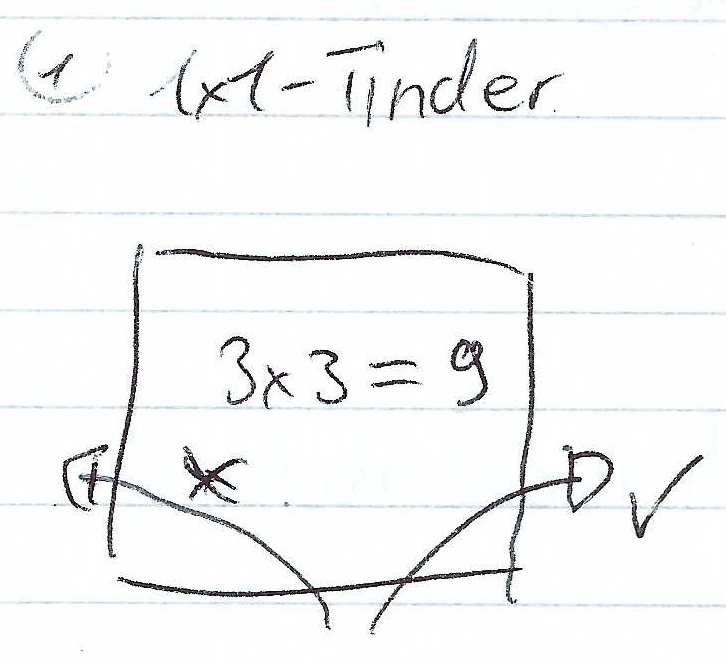
\includegraphics[width=0.5\textwidth]{brainstorming_01_tinder.png}
    \caption{Skizze des Tinder-Ansatzes}
  \end{figure}

  \item Zum richtigen Ergebnis kommen mit viel Tippen unter Zeitdruck
  
  \begin{figure}[h]
    \centering
    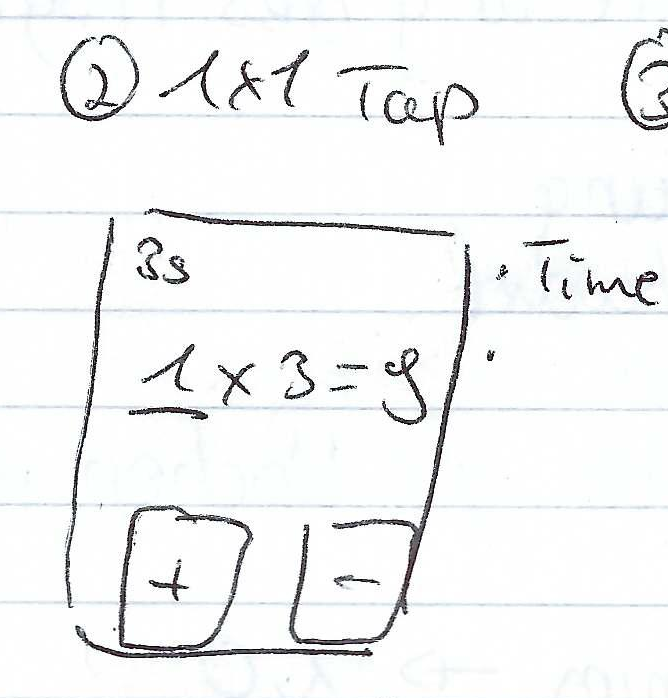
\includegraphics[width=0.5\textwidth]{brainstorming_02_tap.png}
    \caption{Skizze des Tipp-Ansatzes}
  \end{figure}

  \item Rechenaufgaben in interessanten Verkleidungen
  \item Hexagon-Kombinationsspiel á la Dorfromantik
  
  \begin{figure}[h]
    \centering
    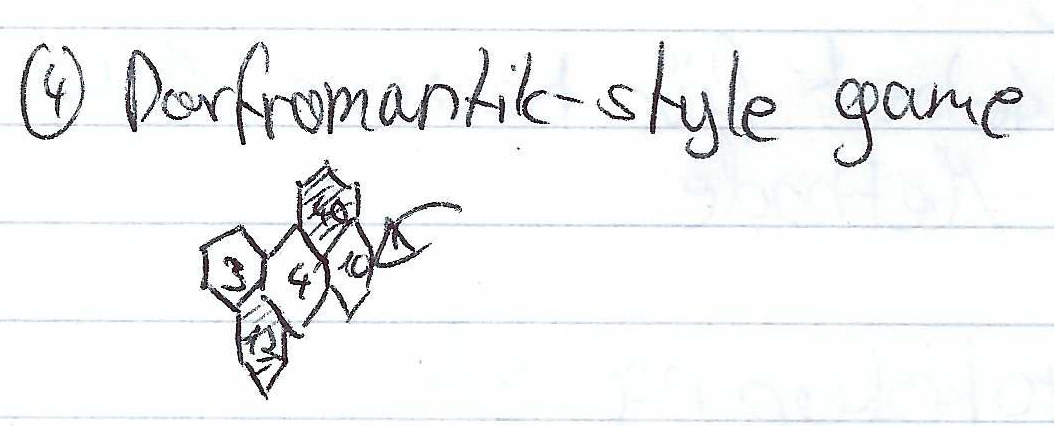
\includegraphics[width=0.5\textwidth]{brainstorming_04_dorfromantik.png}
    \caption{Skizze des \enquote*{Dorfromantik}-Ansatzes}
  \end{figure}

  \item Kombinationsspiel nach dem Vorbild von 2048
  \item Action-reiches Kombinationsspiel mit Geschick und Zeitdruck
  
  \begin{figure}[h]
    \centering
    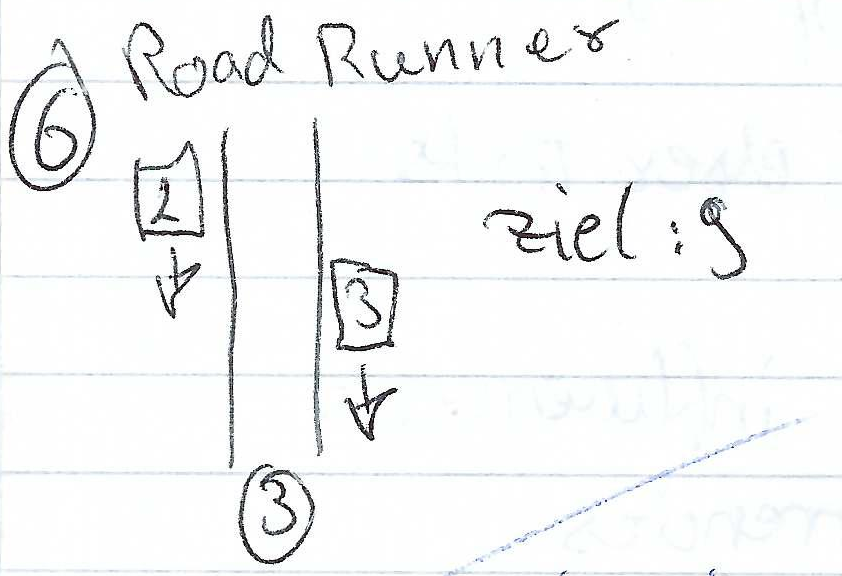
\includegraphics[width=0.5\textwidth]{brainstorming_06_road_runner.png}
    \caption{Skizze des \enquote*{Road Runner}-Ansatzes}
  \end{figure}
\end{enumerate}

\section{1 x 1 Mobile-App}

\subsection{Features}

\subsection{Design}

\subsection{Struktur}

\subsection{Tests}

\section{Ausblick}
